\documentclass{article}
\usepackage[UTF8]{ctex}
\usepackage{geometry}
\usepackage{makecell}
\usepackage{amsmath}
\usepackage{graphicx}
\usepackage{subcaption}
\usepackage{bigstrut}

\geometry{a4paper,scale=0.75}

\title{\heiti 实验八\ 测定金属的杨氏模量}
\author{\kaishu 田睿轩\ 物理学院\ 1900011602}
\date{2021年3月25日}
\newcommand{\degree}{^\circ}
\newcommand{\degreesCelsius}{^\circ C}

\begin{document}
    \maketitle
    \section{数据及处理}
    \subsection{CCD成像测定金属的杨氏模量}
    \subsubsection{实验原理}
    根据胡克定律,材料在弹性限度内,正应力大小$\sigma$与应变$\epsilon$成正比,
    其中,比例系数$E$称为材料的杨氏模量,正应力$\sigma=F/S$,应变$\epsilon=\delta L/L$。
    材料的杨氏模量可以表达为
    $$E=\frac{FL}{S\delta L}$$

    本实验中,通过测量金属丝在受到一定的力$F$而发生拉伸时的形变量$\delta L$,从而测得金属的杨氏模量。
    \subsubsection{实验过程}
    实验装置如图figure1所示,由金属丝和支架、显微镜、CCD相机三部分组成。支架上夹持着一根金属丝,金属丝下端
    连接一小圆柱,小圆柱下端悬挂一个砝码托,通过增减砝码来改变金属丝受到的拉力。圆柱中部的方形窗有细线可供读数,
    细线的移动可以通过显微镜及其内部的分划板上的刻度来观察、测量。为便于读数,使用CCD相机拍摄显微镜的成像画面。

    \begin{figure*}[htb]
        \centering
        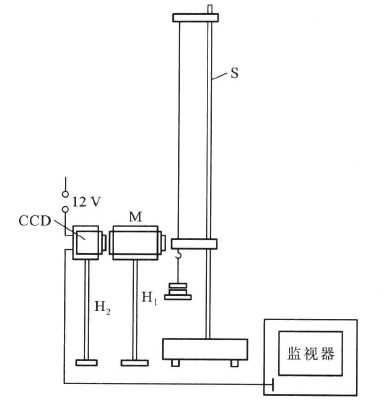
\includegraphics[width=0.3\textwidth]{CCD实验装置.jpg}
        \caption{figure1:CCD成像法实验装置}
    \end{figure*}

    实验中,用刻度尺测量金属丝的原长$L$,用螺旋测微仪测量金属丝的直径$d$从而计算金属丝的横截面积,用天平
    测量砝码质量$m$从而获知金属丝所受拉力,用显微镜测量圆柱的下降距离即金属丝的伸长量$\delta L$。

    \subsubsection{实验数据及处理}
    实验中,用螺旋测微仪测量金属丝不同位置的直径,结果如下表所示
    \begin{center}
        \begin{tabular}{|c|c|c|c|c|c|c|c|c|c|c|c|}
            \hline
            $i$   & 1.0   & 2.0   & 3.0   & 4.0   & 5.0   & 6.0   & 7.0   & 8.0   & 9.0   & 10.0  & $\bar{d'}/mm$ \\
            \hline
            $d_i/mm$ & 0.325  & 0.321  & 0.322  & 0.322  & 0.318  & 0.321  & 0.320  & 0.318  & 0.320  & 0.318  & 0.3205 \\
            \hline
        \end{tabular}%  
    \end{center}

    螺旋测微仪的零点刻度$d_0=-0.005mm$,故金属丝的半径为$\bar{d}=\bar{d'}-d_0=0.321mm$。

    金属丝直径的不确定度包括十次数据的标准差和仪器允差两部分。仪器允差取最小分度值$e=0.01mm$,$\sigma_{d'}=e/\sqrt{3}=5.733\times 10^{-3}mm$,
    标准差$\sigma_{\bar{d}}=\sqrt{\frac{\sum_{i=1}^{10} (d_i-\bar{d})^2}{n(n-1)}}=0.702\times 10^{-3}mm$。因此,直径$d$的不确定度为
    $\sigma_d=\sqrt{\sigma_{\bar{d}}^2+\sigma_{d'}^2}=0.006mm$。

    所以,金属丝直径的测量结果为:
    $$d=(0.321\pm0.006)mm$$

    用刻度尺测得金属丝的长度$L=102.40-23.55=78.85cm$。

    金属丝长度$L$的不确定度主要来自于仪器允差。仪器的允差取其最小分度$e=0.1cm$,因此不确定度为$\sigma_L=0.1/\sqrt{3}=0.06cm$。

    因此,金属丝长度测量结果为:
    $$L=(78.85\pm0.06)cm$$

    实验中测得的砝码的质量及相应的圆柱下降位置如下表所示:

    \begin{center}
        \begin{tabular}{|c|c|c|c|c|c|c|}
            \hline
            $i$     & $m_i$    & $r_i/mm$ & $r'_i/mm$ & $\bar{r_i}/mm$ & $\delta_{m_i}=m_i-m_{i-4}/g$ & $\delta_{r_i}=\bar{r_{i-4}}-\bar{r_i}/mm$ \bigstrut\\
            \hline
            0  & 0.00  & 3.89  & 3.86  & 3.875 & -- & -- \bigstrut\\
            \hline
            1  & 100.38  & 3.83  & 3.78  & 3.805 & -- & -- \bigstrut\\
            \hline
            2  & 300.00  & 3.66  & 3.67  & 3.665 & -- & -- \bigstrut\\
            \hline
            3  & 500.31  & 3.54  & 3.55  & 3.545 & -- & -- \bigstrut\\
            \hline
            4  & 700.23  & 3.43  & 3.44  & 3.435 & -- & -- \bigstrut\\
            \hline
            5  & 899.86  & 3.31  & 3.32  & 3.315 & -- & -- \bigstrut\\
            \hline
            6  & 1099.77  & 3.19  & 3.20  & 3.195 & -- & -- \bigstrut\\
            \hline
            7  & 1299.82  & 3.07  & 3.09  & 3.080 & 799.51 & 0.465 \bigstrut\\
            \hline
            8  & 1499.76  & 2.95  & 2.97  & 2.960  & 799.53 & 0.475 \bigstrut\\
            \hline
            9  & 1699.48  & 2.84  & 2.85  & 2.845 & 799.62 & 0.470 \bigstrut\\
            \hline
            10  & 1899.47  & 2.72  & 2.72  & 2.720 & 799.70 & 0.475 \bigstrut\\
            \hline
        \end{tabular}% 
    \end{center}

   下面分别用逐差法和最小二乘法对数据进行处理

    \textbf{逐差法}
    
    由于$m_i$的间隔是不等的,因此要对$m_i$和$\bar{r_i}$同时进行逐差。考虑到前两个砝码放上去后的圆柱的下降距离
    不能完全反映金属丝的伸长量,又考虑到逐差法需要数据个数尽可能为偶数来保证没有一组数据被消去,因此我们社区$i=0,1,2$的数据,
    然后从$i=3$开始隔5项进行逐差。然后对四个逐差结果取平均。由此可得$m$和$\delta L$的测量结果为:
    $$m=\frac{\delta_{m_7}+\delta_{m_8}+\delta_{m_9}+\delta_{m_10}}{4}=799.59g$$
    $$\delta L=\frac{\delta_{r_7}+\delta_{r_8}+\delta_{r_9}+\delta_{r_10}}{4}=0.47mm$$

    代入杨氏模量的计算公式,可得:
    $$E=\frac{4mgL}{\pi d^2 \delta L}=\frac{4\times 799.59 \times 9.8 \times 0.7885}{\pi \times (0.321\times 10^{-3})^2 \times 0.47}=1.621\times 10^{11}Pa$$

    下面计算逐差法所得的杨氏模量的不确定度。上述对$m$和$\delta L$应用逐差法的过程,本质上也是一种取平均的过程,因此这两个物理量的不确定度
    都包括数据的标准差和仪器误差。

    砝码质量的仪器允差取天平的最小分度值$e=0.01g$,其导致的不确定度$\sigma_{m'}=e/\sqrt{3}=5.77\times 10^{-3}g$。
    数据的标准差$\sigma_{\bar{m}}=\sqrt{\frac{\sum_{i=1}^{4} (m_i-\bar{m})^2}{n(n-1)}}=0.0438g$。因此,质量的不确定度为
    $$\sigma_m=\sqrt{(\sigma_{\bar{m}})^2+(\sigma_m')^2}=0.04g$$

    $\delta L$测量过程中仪器允差取最小分度$e=0.05mm$,其导致的不确定度$\sigma_{\delta L'}=e/\sqrt{3}=0.03mm$。数据的标准差
    $\sigma_{\bar{\delta L}}=\sqrt{\frac{\sum_{i=1}^{4} (r_i-\bar{r})^2}{n(n-1)}}=2.394\times 10^{-3}mm$。因此,$\delta L$的不确定度为
    $$\sigma_{\delta L}=\sqrt{(\sigma_{\bar{\delta L}})^2+(\sigma_{\delta L}')^2}=0.029mm$$

    根据误差传递公式可得杨氏模量的不确定度:
    $$\frac{\sigma_E}{E}=\sqrt{(\frac{\sigma_m}{m})^2+(\frac{\sigma_L}{L})^2+(\frac{2\sigma_d}{d})^2+(\frac{\sigma_{\delta_L}}{\delta_L})^2}$$
    $$\frac{\sigma_E}{E}=1.621\times 10^{11} \sqrt{(\frac{0.04}{799.59})^2+(\frac{0.03}{0.471})^2+(\frac{2\times 0.006}{0.321})^2+(\frac{0.06}{78.85})^2}=0.120\times 10^{11}Pa$$

    综上,逐差法计算杨氏模量的结果为:
    $$E=(1.621\pm 0.12)\times 10^{11}Pa$$



    \textbf{最小二乘法}

    对测得的圆柱位置与砝码质量的关系用最小二乘法进行拟合。由于金属丝在未被拉伸时有一定弯折,因此刚挂上去的砝码
   起到了将金属丝拉直的作用,因此i=0,1时的数据可能不满足胡克定律。所以拟合时舍弃前两组数据,使用剩下的9组数据进行拟合,
   拟合结果如下图figure2所示:
   
   %\newpage
   \begin{figure*}[htb]
        \centering
        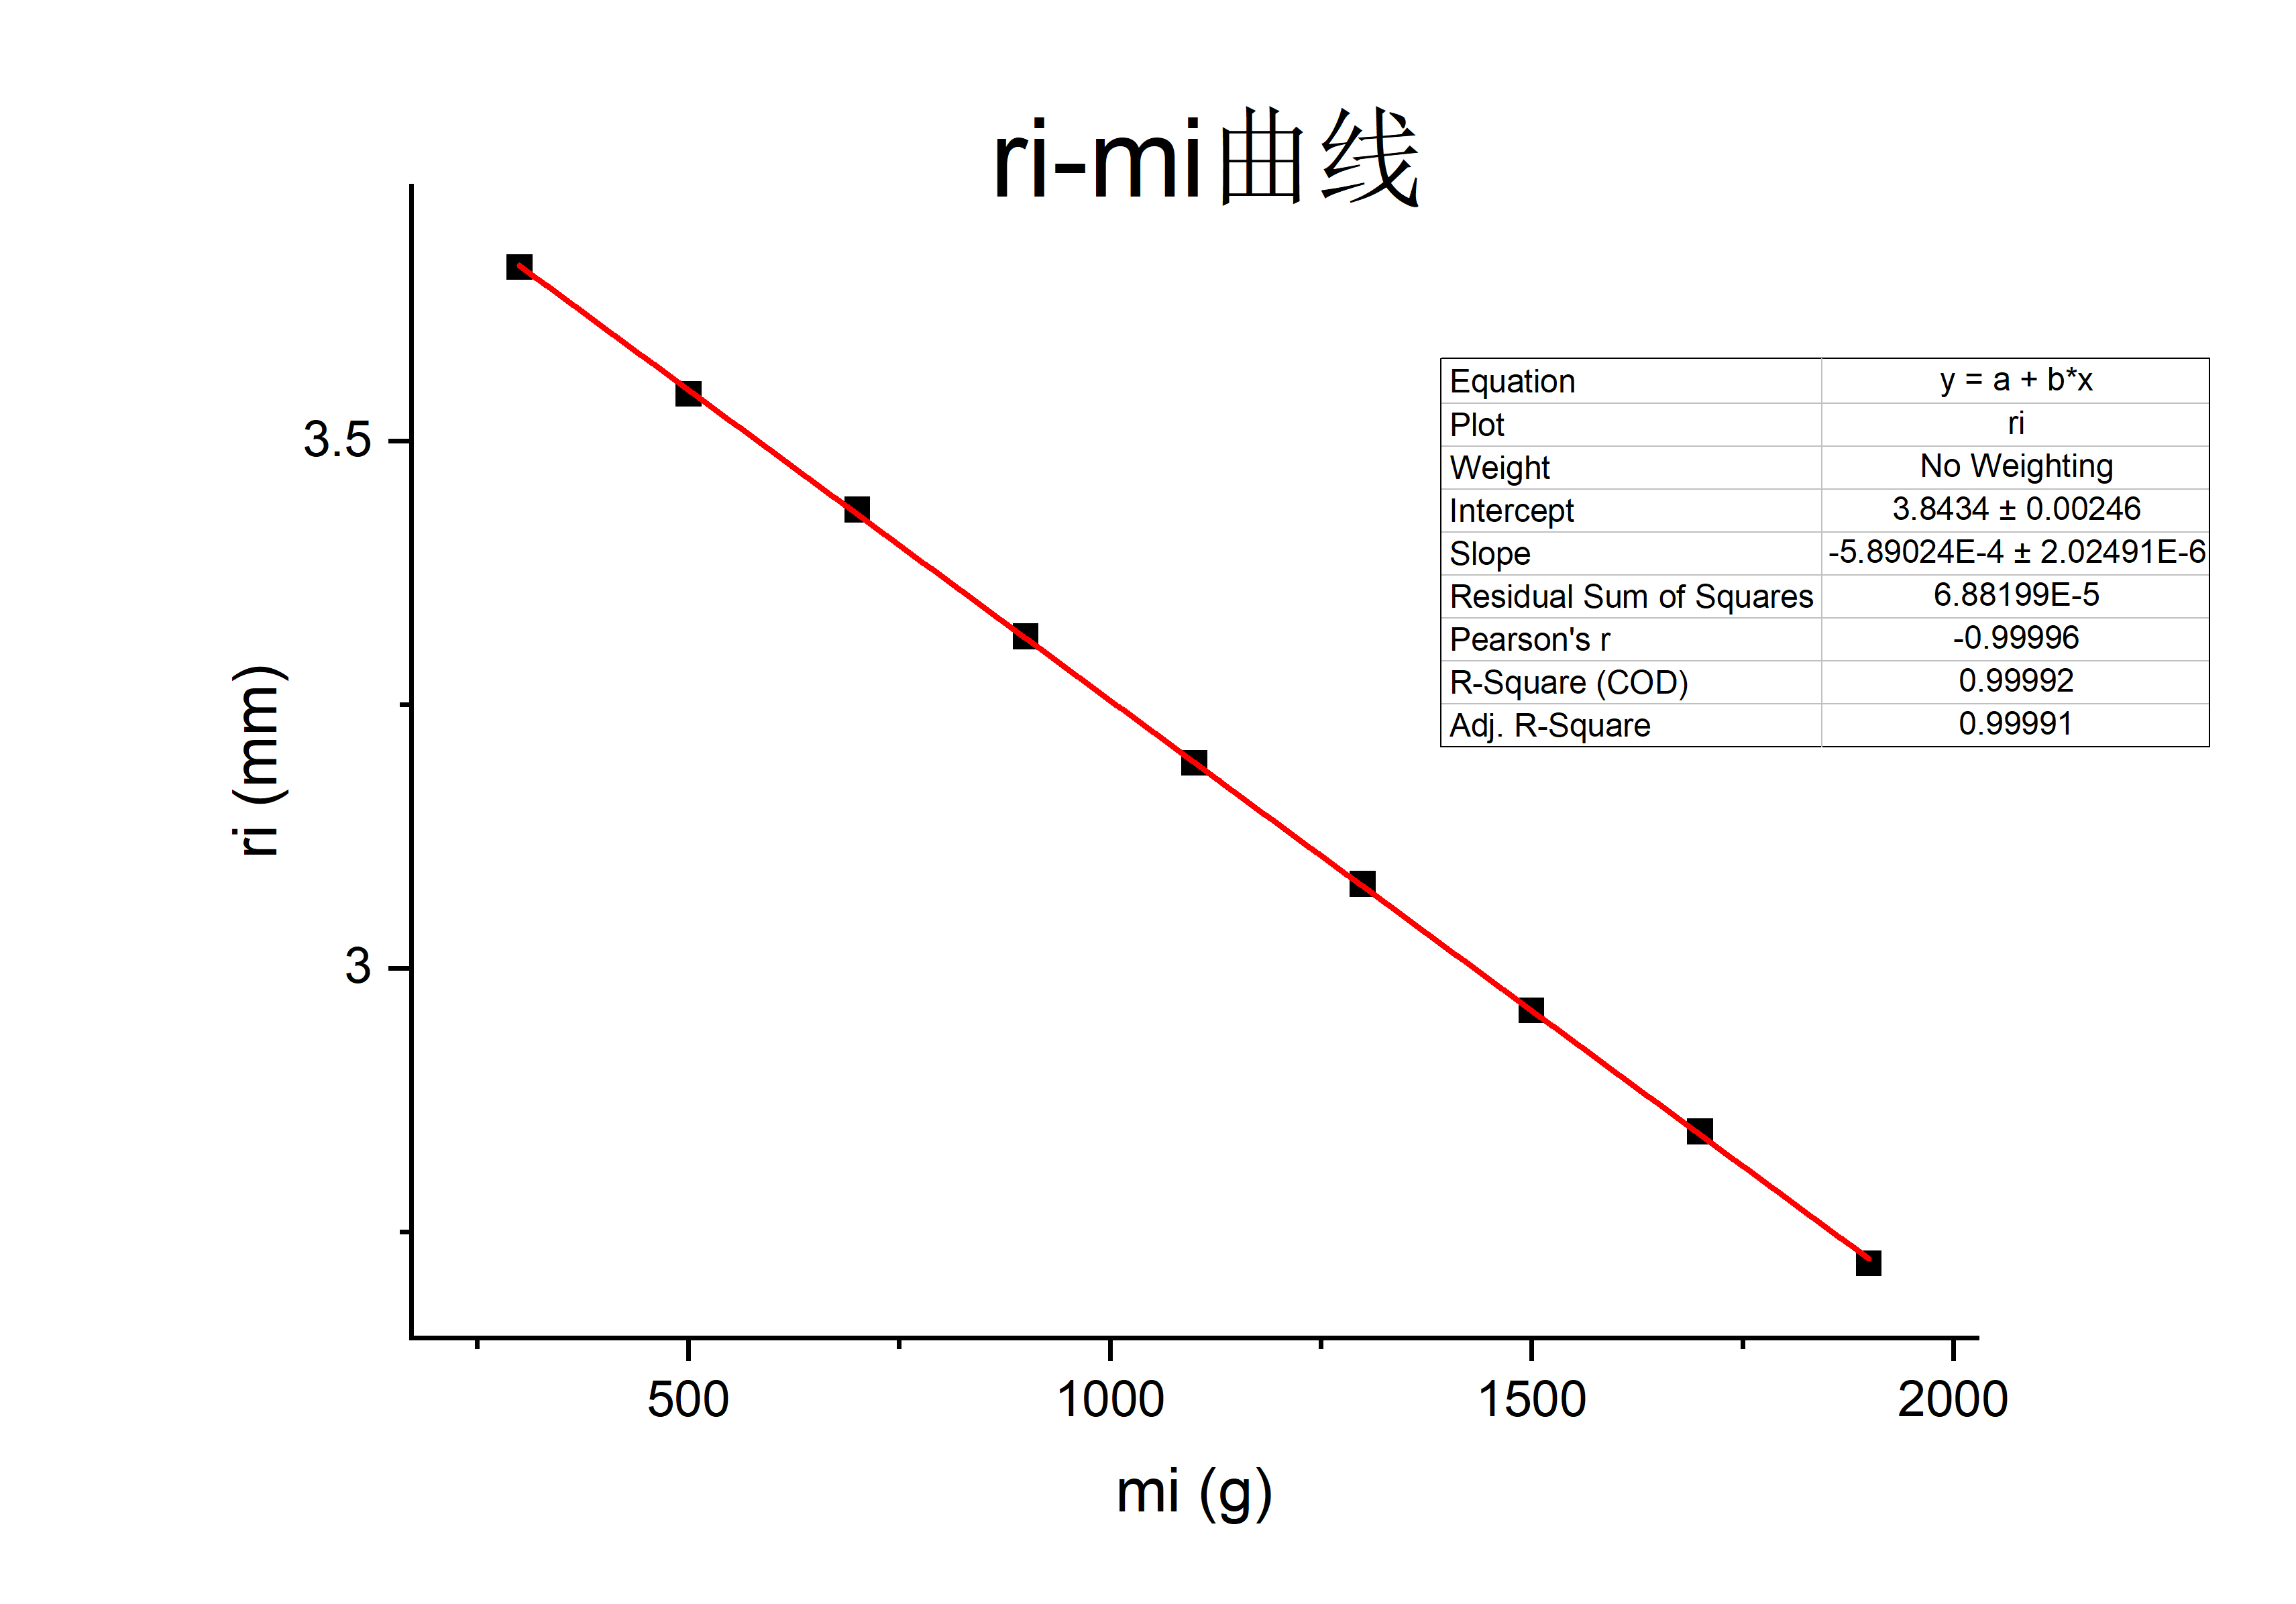
\includegraphics[width=0.8\textwidth]{CCD成像法拟合曲线.jpg}
        \caption{figure2:CCD成像法拟合结果}
    \end{figure*}

    拟合结果斜率的绝对值$|k|=5.890\times 10^{-4}m/kg$,相关系数$r=0.99996$。

    根据$E=\frac{FL}{S\delta L}=\frac{4mgL}{\pi d^2 \delta L}$,可知$\delta L=\frac{4mL}{\pi d^2 E}m$,
    故$r_i-m_i$曲线的斜率的绝对值满足$|k|=\frac{4gL}{\pi d^2 E}$,于是可得杨氏模量$E$的计算公式:
    $$E=\frac{4gL}{\pi d^2 k}=\frac{4\times 9.8\times 0.7885}{\pi \times (0.321\times 10^{-3})^2\times (5.890\times 10^{-4})}=1.621\times 10^{11}Pa$$

    下面计算最小二乘法得出的杨氏模量的不确定度。

    斜率$k$的不确定度包括拟合带来的a类不确定度和来自仪器允差的b类不确定度,其中仪器允差取最小分度$e=0.05mm$。$\sigma_{k,a}=k\sqrt{\frac{1/r^2-1}{n-2}}=5.890\times 10^{-4}\sqrt{\frac{1/0.99996^2-1}{7}}=0.020\times 10^{-4}mm/g$,
    $\sigma_{k,b}=\frac{e/\sqrt{3}}{\sqrt{\sum_{i=1}^9 (x_i=\bar{x})^2}}=\frac{0.05/\sqrt{3}}{\sqrt{2397765}}=0.186\times 10^{-4}mm/g$。$\sigma_k=\sqrt{\sigma_{k,a}^2+\sigma_{k,b}^2}=0.187\times 10^{-4}mm/g$。

    杨氏模量$E$的不确定度由$d,k,L$的不确定度传递而来,
    $$\frac{\sigma_E}{E}=\sqrt{(\frac{\sigma_L}{L})^2+(\frac{2\sigma_d}{d})^2+(\frac{\sigma_k}{k})^2}$$
    $$\sigma_E=1.621\times 10^{11} \sqrt{(\frac{0.06}{78.85})^2+(\frac{2\times 0.006}{0.321})^2+(\frac{0.187}{5.890})}=0.080\times 10^{11}Pa$$

    所以,杨氏模量$E$的测量结果为:
    $$E=(1.621\pm 0.080) \times 10^{11} Pa$$

    \subsection{梁弯曲法测定杨氏模量}
    \subsubsection{实验原理}
    横梁在中部受力时会发生弯曲(如图figure3所示),其挠度$\lambda$在$\lambda \ll l$时满足$\lambda=\frac{mgl^3}{4ah^3E}$,
    其中$l$为横梁有效长度,$a$为横梁宽度,$h$为横梁厚度,$m$为悬挂重物的质量。于是,杨氏模量E可表示为:
    $$E=\frac{mgl^3}{4\lambda ah^3}$$

    本实验通过测量$m,l,a,h,\lambda$来测量金属的杨氏模量

    \begin{figure*}[htb]
        \centering
        \begin{subfigure}[h]{0.52\textwidth}
            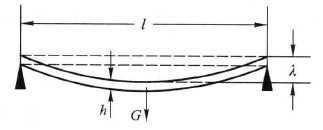
\includegraphics[width=\textwidth]{梁弯曲法原理图.jpg}
            \caption{figure3:梁弯曲法原理图}
        \end{subfigure}
        \begin{subfigure}[h]{0.44\textwidth}
            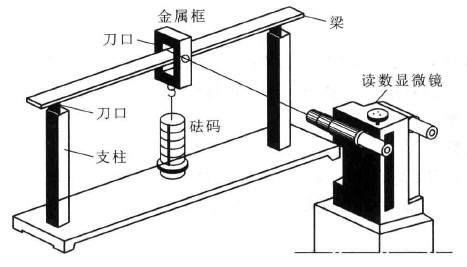
\includegraphics[width=\textwidth]{梁弯曲发装置图.jpg}
            \caption{figure4:梁弯曲法装置图}
        \end{subfigure}
    \end{figure*}

    \subsubsection{实验过程}
    实验装置如figure4所示,横梁架在两个支架上的刀口上,横梁中部用刀口支撑一个金属架,金属架下方悬挂一个砝码托,
    用增减砝码的方式改变配重。用刻度尺测量横梁的有效长度(两刀口之间的长度)、用游标卡尺测量横梁宽度,
    用螺旋测微仪测量横梁厚度。用天平测量砝码质量,用读数显微镜观察并测量梁的下降距离即挠度。

    \subsubsection{实验数据及处理}
    实验中测得横梁的有效长度为$l=20.10cm$,不确定度$\sigma_l=\frac{e}{\sqrt{3}}=0.1/\sqrt{3}=0.06cm$。宽度为$a=1.010cm$,
    其不确定度$\sigma_a=\frac{e}{\sqrt{3}}=0.005/\sqrt{3}=0.003cm$。厚度的测量结果如下表所示:

    \begin{center}
        \begin{tabular}{|c|c|c|c|c|c|c|c|c|c|c|c|}
            \hline
            i     & 1     & 2     & 3     & 4     & 5     & 6     & 7     & 8     & 9     & 10    & $\bar{h'}/mm$ \bigstrut\\
            \hline
            $h_i/mm$ & 1.535 & 1.542 & 1.542 & 1.528 & 1.525 & 1.508 & 1.52  & 1.48  & 1.538 & 1.536 & 1.524 \bigstrut\\
            \hline
        \end{tabular}%            
    \end{center}

    实验中螺旋测微仪的零点值为$h_0=-0.010mm$,因此横梁的厚度为$\bar{h}=1.524+0.010=1.534mm$。

    实验中所测得砝码质量及相应的梁挠度如下表所示:
    \begin{center}
        \begin{tabular}{|c|c|c|c|c|c|c|}
            \hline
            i     & $m_i/g$ & $r_i/mm$ & $r'_i/mm$ & $\bar{r_i}/mm$ & $\delta m_i = m_i-m_{i-3}/g$ & $\delta L_i=\bar{r_{i-3}}-\bar{r_{i}}/mm$  \bigstrut\\
            \hline
            0     & 0.00     & 46.209 & 46.178 & 46.1935 & -- & -- \bigstrut\\
            \hline
            1     & 200.12 & 45.68 & 45.654 & 45.6670 & -- & -- \bigstrut\\
            \hline
            2     & 399.8 & 45.165 & 450138 & 45.1515 & -- & -- \bigstrut\\
            \hline
            3     & 599.63 & 44.634 & 44.618 & 44.6260 & -- & -- \bigstrut\\
            \hline
            4     & 799.36 & 44.119 & 44.1  & 44.1095 & 599.24 & 1.5575\bigstrut\\
            \hline
            5     & 999.34 & 43.573 & 43.571 & 43.5720 & 599.54 & 1.5795\bigstrut\\
            \hline
            6     & 1199.22 & 43.044 & 43.044 & 43.0440 & 599.59 & 1.5820\bigstrut\\
            \hline
        \end{tabular}%
    \end{center}

    下面用逐差法和最小二乘法分别对结果进行处理。

    \textbf{逐差法}

    舍弃第一组数据,然后对后面三组数据隔三项进行逐差,然后对结果取平均
    $$m=\frac{\delta m_4+\delta m_5 + \delta m_6}{3}=599.46g$$
    $$\delta L=\frac{\delta L_4+\delta L_5+\delta L_6}{3}=1.573mm$$

    代入杨氏模量的计算公式,可得:
    $$E=\frac{mgl^3}{4\lambda ah^3}=\frac{599.46\times 9.8 \times 0.201^3}{4\times 1.573\times0.0101\times (1.534\times 10^{-3})^3}=2.080\times 10^{11} Pa$$

    \textbf{最小二乘法}
    
    最小二乘法拟合结果如下图figure5所示:

    \begin{figure*}[htb]
        \centering
        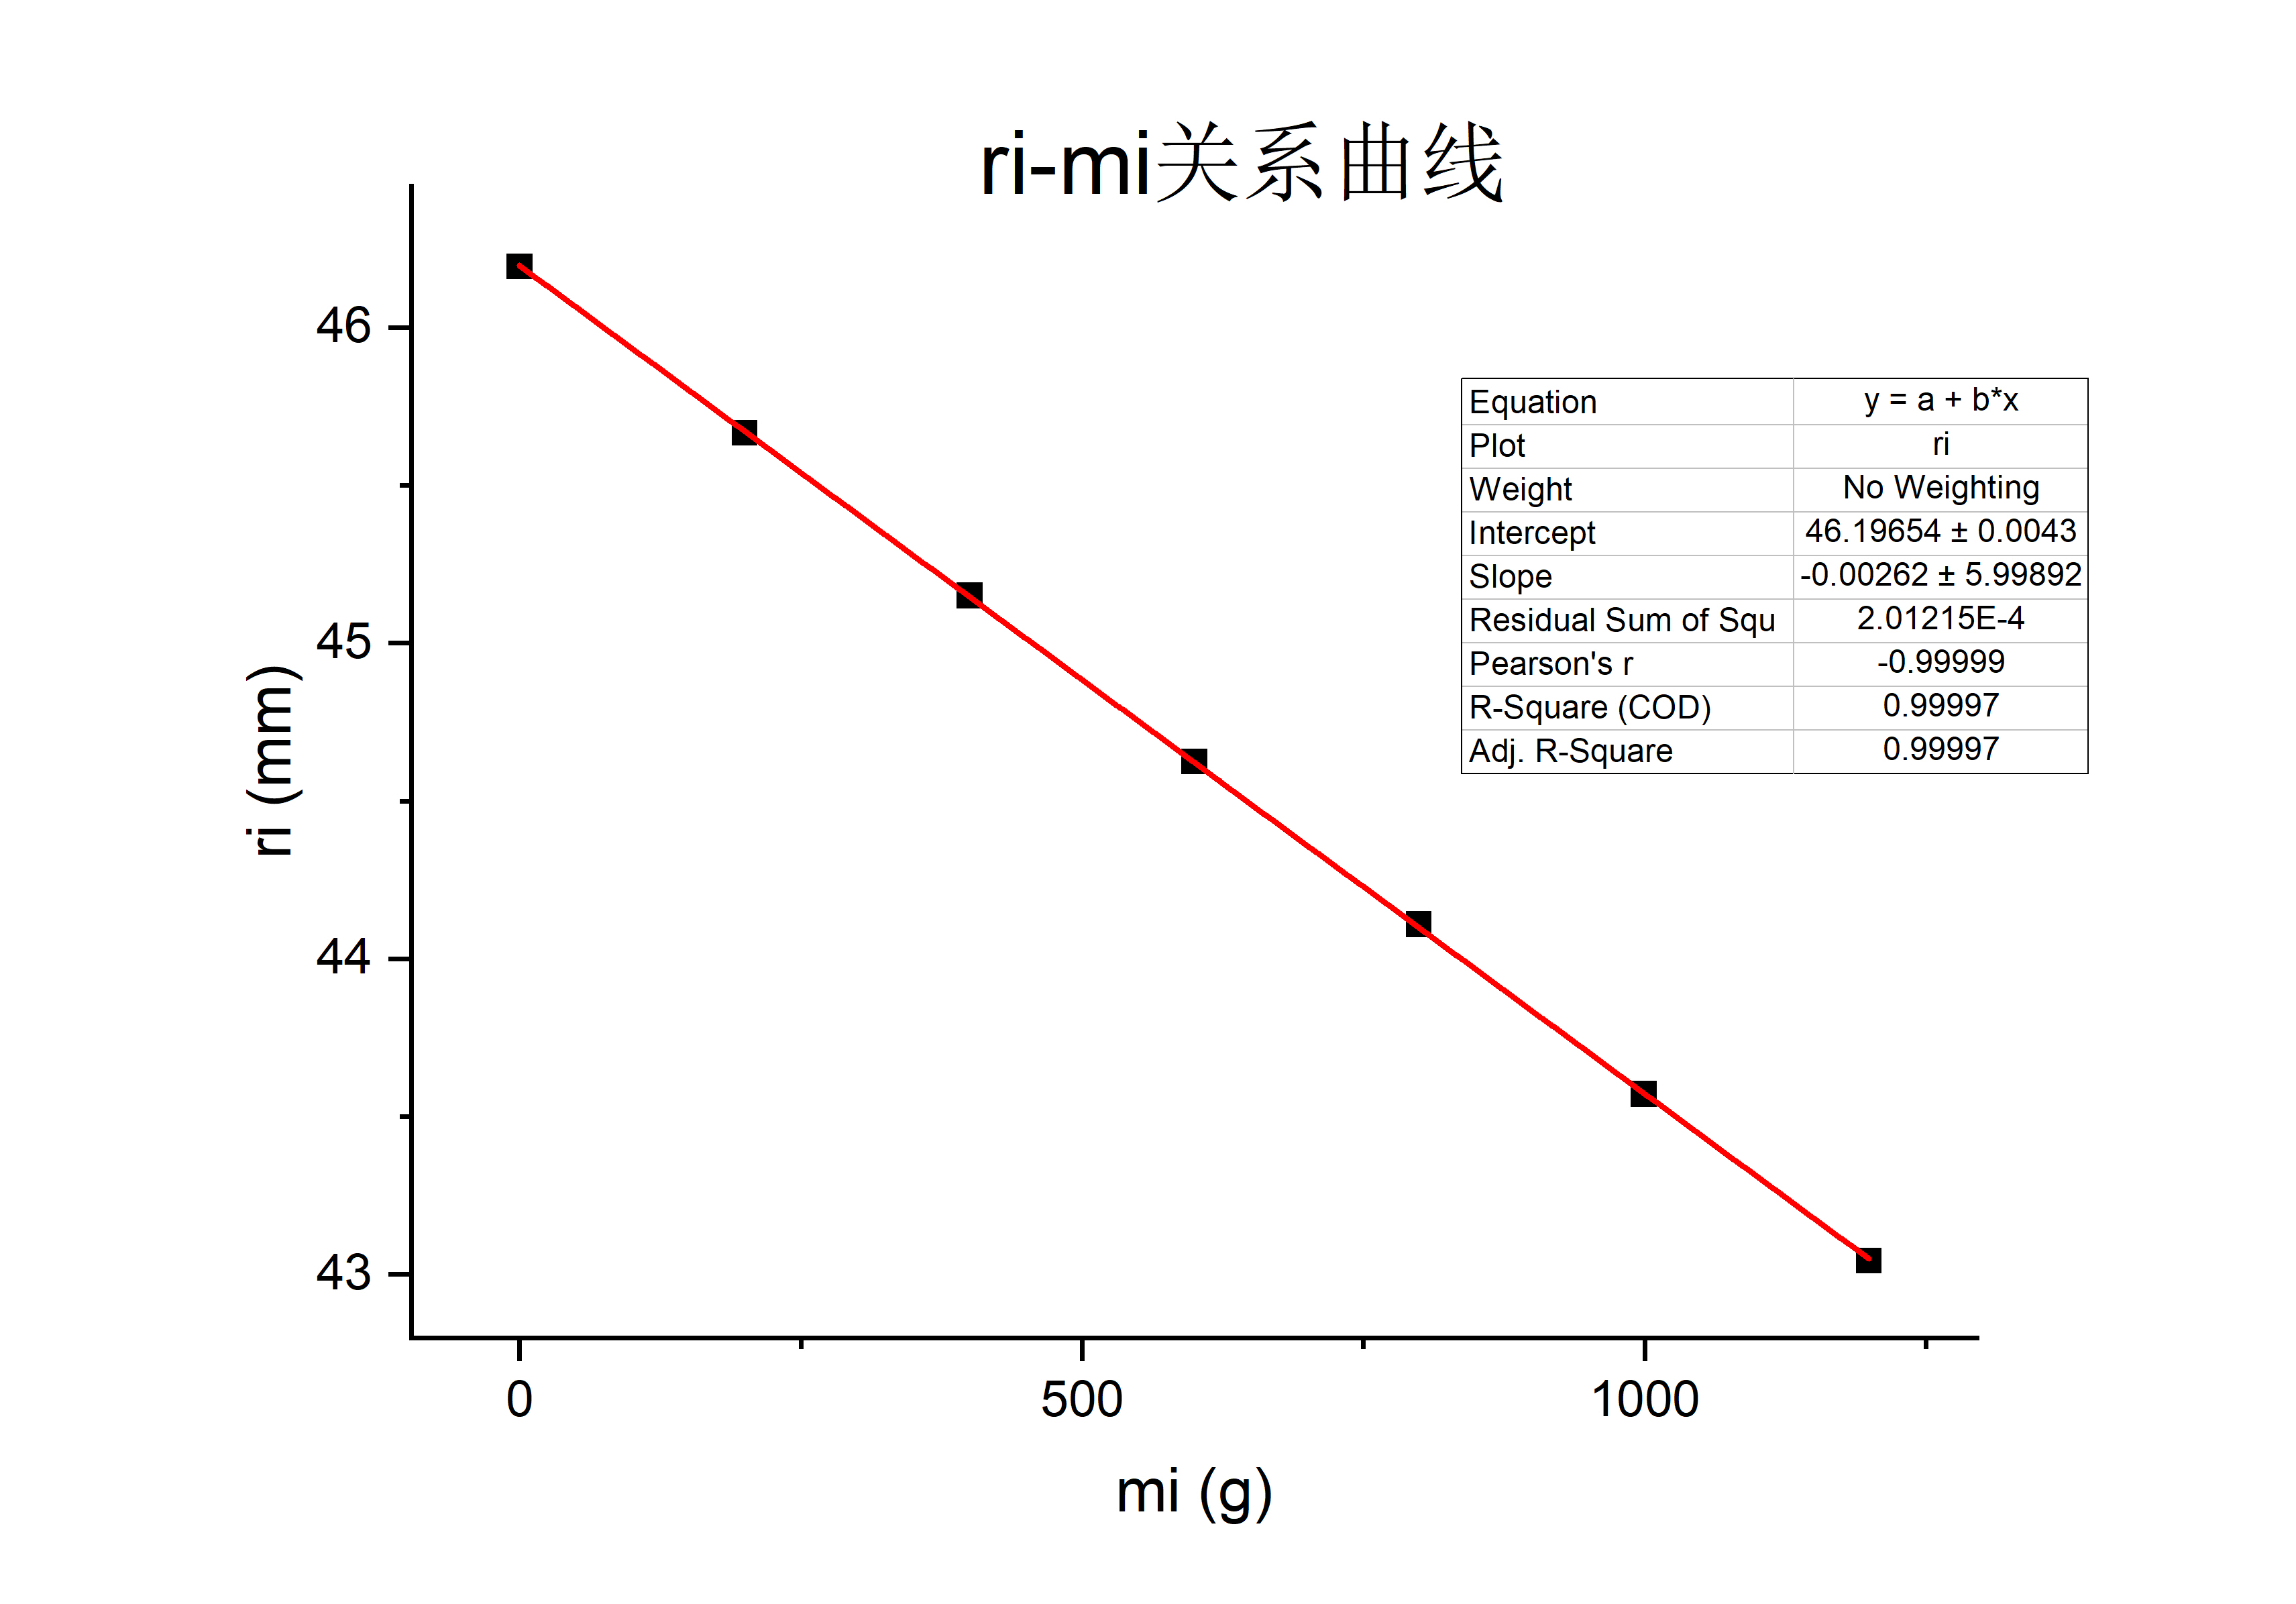
\includegraphics[width=0.8\textwidth]{梁弯曲法拟合结果.jpg}        
        \caption{figure5:梁弯曲法拟合结果}
    \end{figure*}

    其中,斜率的绝对值$|k|=2.624\times 10^{-3}mm/g$,相关系数$r=0.99999$。

    由于杨氏模量满足表达式$E=\frac{mgl^3}{4\lambda ah^3}$,因此挠度与砝码质量之间存在
    关系$\lambda=\frac{mgl^3}{4ah^3E}$,所以曲线斜率的绝对值可表示为$|k|=\frac{gl^3}{4ah^3E}$,
    故可计算得杨氏模量
    $$E=\frac{gl^3}{4ah^3|k|}=\frac{9.8\times 0.201^3}{4\times (1.01\times 10^{-2})\times (1.534\times 10^{-3})^3 \cdot 2.624\times 10^{-3}}=2.080\times 10^{11} Pa$$

    \section{分析与讨论}
    针对开始加砝码时$r$的变化量大于或小于正常变化量的情况,有以下推测:

    $r$的变化量大于正常变化量:可能是因为金属丝发生了弯曲,刚加上去的砝码除了使金属丝发生伸长的应变外,
    还使金属丝由弯变直,这部分的长度变化量就是多出来的变化量

    $r$的变化量小于正常变化量:可能是因为金属丝下方的圆柱与限位螺丝之间有摩擦
\end{document}